\documentclass[11pt]{article}
\usepackage[a4paper,margin=1in]{geometry}
\usepackage{amsmath,amssymb,amsthm,mathtools}
\usepackage{booktabs}
\usepackage{enumitem}
\usepackage{graphicx}
\usepackage{hyperref}
\usepackage[nameinlink,capitalise]{cleveref}
\usepackage[numbers,sort&compress]{natbib}

\newtheorem{theorem}{Theorem}[section]
\newtheorem{proposition}[theorem]{Proposition}
\newtheorem{corollary}[theorem]{Corollary}
\theoremstyle{remark}
\newtheorem{remark}[theorem]{Remark}
\newcommand{\norm}[1]{\left\lVert#1\right\rVert}

\title{From Half-Log Rank Clocks to Schur Packet Bootstrap\\
\large A Ten-Layer Review and the Revised Stage-A Frontier}
\author{Liang Wang}
\date{July 2026}

\begin{document}
\maketitle

\begin{abstract}
RH-82--RH-90 pursued the preferred postblock effective-rank corridor from an
endpoint rank clock to a full-reference-free Schur certificate.  This tenth
paper extracts the resulting all-level sufficient theorem, audits the nine
dependencies, and revises the Stage-A/A5 frontier.

For normalized memory Gramians
$G_j=X_j^*X_j/\norm{X_j}_2^2+\eta G_{j-1}$, suppose a nondecreasing
clock-rank law and the RH-90 Schur condition give
$E_{j+1}\le\rho E_j$ for $m$ consecutive late updates, where $E_j$ is the
optimal packet tail and $0<\rho<1$.  The Schur-to-effective-rank bootstrap
theorem gives
\[
 E_{b+m}\le\frac{\rho^m}{1-\eta},\qquad
 \frac{\tau_{r_{b+m}}(X_{b+m})}{\norm{X_{b+m}}_2}
 \le\frac{\rho^{m/2}}{\sqrt{1-\eta}}.
\]
At the audited values $\eta=1/512$ and $\rho=0.24$, 20 updates suffice for a
$10^{-6}$ relative tail and 39 for $10^{-12}$.

The nine archived summaries contain 29 theorem flags, all green in their
stated scopes.  The positive chain is: half-log clock, captured energy,
strict-prefix packet, normalized memory, scalar injection, predictor-corrector
factorization, rank-one Ritz enrichment, and Schur sign.  The branch-specific
negative results rule out coordinate identity, unweighted prefix Gramians,
tail-angle perturbation, global-norm contraction, and uniform point-packet
contraction as shortcuts.

The revised completion frontier is not a claim that Stage A is closed.  Its
two alternatives are the RH-75 full-block law or a three-part Schur packet
bundle: uniform late Schur contraction, polylogarithmic reduced packet future,
and the inherited finite-prefix/normalization/observability bridge.  The A5
moving-cloud projection, coefficient bridge, and uniform complement remain
unchanged.  No Hilbert--Polya or Riemann Hypothesis conclusion is made.
\end{abstract}

\noindent\textbf{Keywords:} effective rank; Schur certificate; dynamic
packet; dependency frontier; validated numerics; small noise.

\medskip
\noindent\textbf{MSC 2020:} 47A75; 47B10; 37C30; 65G20.

\section{How the route changed}

RH-82 sharpened the endpoint resolution theorem to a half-logarithmic
excess-rank tail \citep{WangHalfLog2026}.  RH-83 characterized the optimal
singular factorization while rejecting coordinate identity
\citep{WangFactor2026}.  RH-84 then showed that the downstream problem needs
only captured tail energy, not factorization or termwise singular control
\citep{WangKyFan2026}.

RH-85 constructed a strict-prefix dynamic packet and proved that unweighted
prefix energy can fail \citep{WangSnapshot2026}.  RH-86 introduced a
trace-normalized memory packet and found that principal-angle bounds are
quantitatively unusable \citep{WangMemory2026}.  RH-87 reduced packet drift to
a scalar Rayleigh injection recursion \citep{WangInjection2026}.

RH-88 separated old-packet prediction from variational correction and closed
the global-norm and uniform point-packet shortcuts at the anchors
\citep{WangPredictor2026}.  RH-89 found that one complement direction plus an
$(r+1)$-dimensional Ritz solve recovers almost all reference correction
\citep{WangRitz2026}.  RH-90 replaced that full reference by a directly
validated small Schur sign \citep{WangSchur2026}.

\section{Schur-to-effective-rank bootstrap theorem}

Let
\[
 \widehat G_j=\frac{X_j^*X_j}{\norm{X_j}_2^2},\qquad
 G_j=\widehat G_j+\eta G_{j-1},\qquad G_{-1}=0,
\]
with $0\le\eta<1$.  Let $E_{j,r}$ be the optimal rank-$r$ tail of $G_j$.

\begin{theorem}[Schur-to-effective-rank bootstrap theorem]
\label{thm:bootstrap}
Let $r_j$ be nondecreasing.  Suppose that for $j=b,\ldots,b+m-1$, either the
old packet already meets the target or an RH-90 Schur trial certifies
\begin{equation}
 E_{j+1,r_{j+1}}\le\rho E_{j,r_j},\qquad0<\rho<1.
 \label{eq:contract}
\end{equation}
Then
\begin{align}
 E_{b+m,r_{b+m}}&\le\frac{\rho^m}{1-\eta},
 \label{eq:memory-tail}\\
 \frac{\tau_{r_{b+m}}(X_{b+m})}{\norm{X_{b+m}}_2}
 &\le\frac{\rho^{m/2}}{\sqrt{1-\eta}}.
 \label{eq:snapshot-tail}
\end{align}
Consequently a tolerance $\varepsilon$ is reached once
\[
 m\ge
 \frac{2\log(1/(\varepsilon\sqrt{1-\eta}))}{|\log\rho|}.
\]
\end{theorem}

\begin{proof}
Every $\widehat G_j$ has trace one, hence
$\operatorname{tr}G_b\le\sum_{k=0}^b\eta^k\le(1-\eta)^{-1}$ and
$E_{b,r_b}\le(1-\eta)^{-1}$.  Iterating \eqref{eq:contract} gives
\eqref{eq:memory-tail}.  The current snapshot is a weight-one summand of the
memory objective, so its optimal relative squared residual is at most
$E_{b+m,r_{b+m}}$.  Taking square roots proves \eqref{eq:snapshot-tail} and
the update count.
\end{proof}

\begin{corollary}[Conditional RH-78 residual gate]
Assume the clock rank is $O(\log(1/\sigma))$, the Schur updates in
\cref{thm:bootstrap} persist for the required late window, and
$\sqrt{G_\sigma}\norm{X_\sigma}_2$ is polylogarithmic.  Then the
observability-transferred effective-rank residual is polylogarithmic, and may
be made power-small if the late window is $\Omega(\log(1/\sigma))$.
\end{corollary}

This corollary supplies only the residual term in the RH-78 effective-rank
corridor \citep{WangTwoCorridors2026}.  The reduced packet future and finite
prefix must still be proved polylogarithmic.

\section{Nine-paper ledger and negative markers}

\begin{table}[ht]
\centering
\small
\begin{tabular}{rlll}
\toprule
Paper & Durable object & Route effect & Remaining boundary\\
\midrule
82 & half-log tail & rank clock & physical transfer\\
83 & optimal factorization & strength audit & coordinate no-go\\
84 & Ky Fan tail & weaker invariant & all-level energy\\
85 & prefix packet & dynamic construction & unweighted no-go\\
86 & normalized memory & gap-free online packet & angle no-go\\
87 & injection recursion & scalar reduction & injection law\\
88 & predictor/corrector & correction dividend & norm/point no-go\\
89 & one-direction Ritz & small corrector & cross enrichment\\
90 & Schur trial & reference-free certificate & uniform sign\\
\bottomrule
\end{tabular}
\caption{RH-82--RH-90.  Negative verdicts apply only to the named shortcut.}
\label{tab:ledger}
\end{table}

The five branch-specific negative results are durable route markers, not
global no-go theorems.  In particular, the failure of tail-angle continuity
does not conflict with stable captured energy, and the failure of old-packet
contraction does not conflict with corrected packet contraction.

\section{Validated bootstrap budget}

The review hashes all nine summaries and evaluates the bootstrap at 256-bit
precision with $\eta=1/512$ and $\rho=0.24$.

\begin{table}[ht]
\centering
\small
\begin{tabular}{rrr}
\toprule
relative tolerance & minimal updates & certified bound\\
\midrule
$10^{-2}$ & 7 & $6.779\times10^{-3}$\\
$10^{-4}$ & 13 & $9.372\times10^{-5}$\\
$10^{-6}$ & 20 & $6.347\times10^{-7}$\\
$10^{-8}$ & 26 & $8.774\times10^{-9}$\\
$10^{-10}$ & 33 & $5.942\times10^{-11}$\\
$10^{-12}$ & 39 & $8.214\times10^{-13}$\\
\bottomrule
\end{tabular}
\caption{Minimality is certified by checking that the preceding update remains
above the requested tolerance.}
\label{tab:budget}
\end{table}

The count is logarithmic in inverse tolerance.  It does not show that the
Schur sign persists for 39 physical updates; that persistence is precisely
the new all-level theorem wall.

\begin{figure}[ht]
\centering
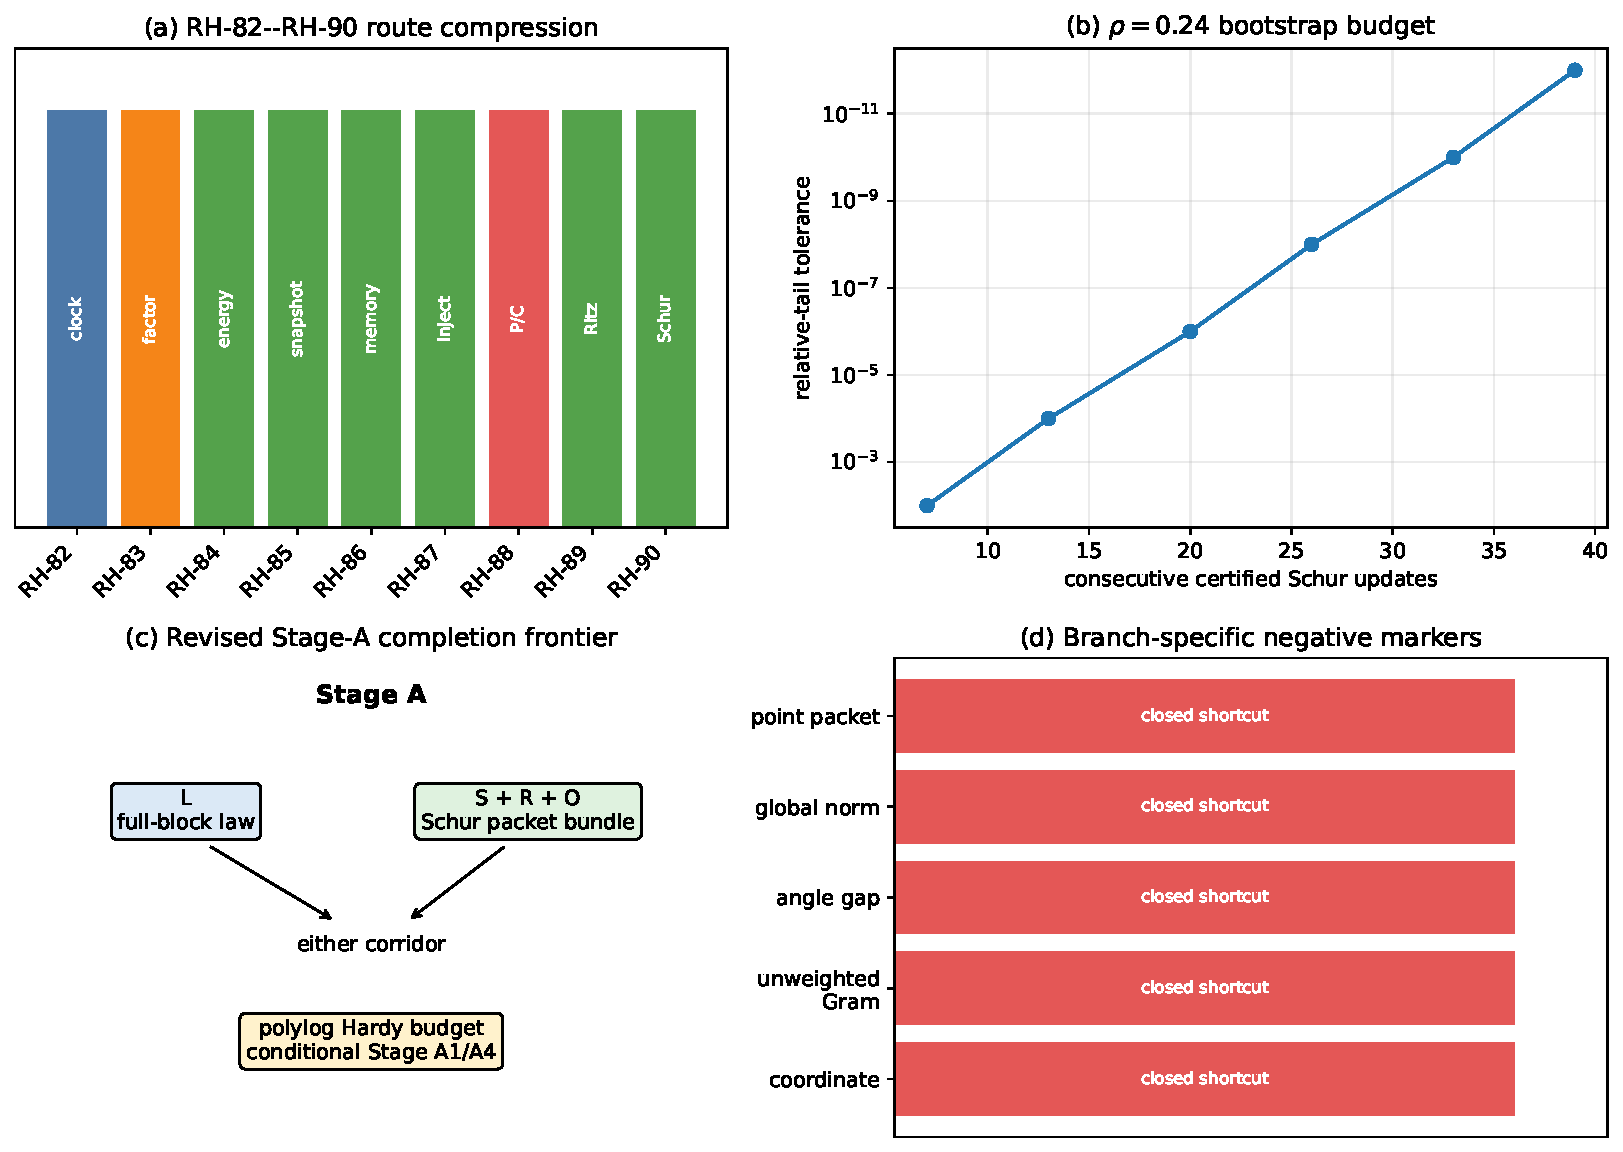
\includegraphics[width=\textwidth]{figures/schur_packet_route_review.pdf}
\caption{The nine-layer compression, contraction budget, revised Stage-A
frontier, and branch-specific negative markers.}
\label{fig:review}
\end{figure}

\section{Revised completion frontier}

Let $L$ be the all-level full-block law, $S$ the uniform late Schur update
law, $R$ the polylogarithmic reduced packet future, and $O$ the inherited
finite-prefix/normalization/observability bridge.  With the finite chain
closed in its archived scope, the revised sufficient Stage-A formula is
\[
 \mathsf A_1= L\ \vee\ (S\wedge R\wedge O).
\]
Its minimal open bundles are $\{L\}$ and $\{S,R,O\}$.  This is the revised
completion frontier: RH-82--90 greatly sharpen $S$, but do not prove $S$, $R$,
or $O$ uniformly.

For relative A5, append the unchanged moving-cloud gates $P,C,U$ from RH-81
\citep{WangRouteReview2026}.  The two sufficient bundles become
\[
 \{L,P,C,U\},\qquad\{S,R,O,P,C,U\}.
\]
No canonical scattering completion, self-adjoint generator, intrinsic
$T\log T$ law, prime-power trace formula, completed-zeta identity,
Hilbert--Polya operator, zeta-zero identification, or Riemann Hypothesis
result is established here.

\bibliographystyle{plainnat}
\bibliography{references}

\end{document}
